\documentclass[a4paper, 10pt]{article}

\usepackage{cite}
\usepackage{color}
	\definecolor{gray}{rgb}{0.5,0.5,0.5}
\usepackage{fancyvrb}
\usepackage{graphicx}
\graphicspath{{images/}}
\DeclareGraphicsExtensions{.pdf,.png}
\usepackage{hyperref}
\usepackage{listings}
	\lstset{
		frame=single,
		numbers=left,
		numberstyle=\small\color{gray},
		tabsize=4,
	}
\usepackage{multirow}
\usepackage{setspace}
\usepackage{url}

\hyphenation{op-tical net-works semi-conduc-tor}

\def \todo#1{\textcolor{blue}{#1}}

\title{A Different Barrier}
\author{Ronny Brendel}

\begin{document}
\maketitle

\begin{abstract}
	In this report I present a new barrier protocol, that does not need locking mechanisms nor atomic operations. I prove its termination by means of checking appropriate properties on a markov decision process model. Furthermore the results of a quantitative analysis on a continuous-time markov chain model of the protocol will be evaluated. Moreover I present implementation and evaluate its performance in comparison to current barrier implementations. To conclude the report I repeat the main points and achievements of the work, and give a perspective on possible next steps.
\end{abstract}

%%%%%%%%%%%%%%%%%%%%%%%%%%%%%%%%%%%%%%%%%%%%%%%%%%%%%%%%%%%%%%%%%%%%%%%%%%%%%%%
\section{Introduction}
Inspired by the idea of pW/CS\cite{pwcs} we intend to evaluate which other synchronisation operations can be improved through stochastic algorithms. One of those operations is the barrier.

A barrier is a synchronisation primitive where all processes in a team wait until all of them reach this barrier. \cite{hoefler2005} gives a good overview and analysis of current barrier protocols.

The barrier is a common synchronisation operation. In OpenMP\cite{omp} by default many operations such as for loops, sections, single directives invoke an implicit barrier at the end of the operation. Many distributed computing algorithms use a \emph{lock-step} approach to interleave computation with communication phases. For example a program simulating weather divides the region in question into a grid. In each of the squares on this grid the weather progression of the next 20 seconds is simulated concurrently. As a next step the squares need to exchange information such as the temperature and humidity at the borders to the neighbouring squares in order to be able to simulate the next 20 seconds. To facilitate this behaviour barriers are used to make sure all squares have been simulated and are ready to exchange data, before repeating this process.

According to a survey conducted at the HLRS\footnote{url{http://http://www.hlrs.de}}\cite{rab00} the barrier is the 5th most time-consuming MPI\footnote{short for Message Passing Interface}\cite{mpi} operation. On average 6\% of the whole CPU time spent in MPI calls and 0.81\% of the whole program time is spent in barriers. A very small fraction of this is the actual time spent synchronizing. The majority is due to waiting for other processes to arrive, because the computation between processes is unbalanced - some take longer, some are quicker. It is still useful to pursue improvements in the barrier protocol for benchmarks and programs that require a lot of synchronisation.

The report is structured as follows. First I present the new protocol. After this I prove its correctness/termination. The next step is to analyse quantitative properties of the protocol. Furthermore an implementation will be evaluated and compared to the barrier implementations of GNU OpenMP\cite{gomp} and PThreads\cite{glibc} implementation.

%%%%%%%%%%%%%%%%%%%%%%%%%%%%%%%%%%%%%%%%%%%%%%%%%%%%%%%%%%%%%%%%%%%%%%%%%%%%%%%
\section{A lockless shared memory barrier without atomic operations}
The protocol depicted in figure~\ref{fig:barrier-source-code} went through multiple iterations. Therefore it is not immediately obvious why there are two distinct loops and what the purpose of the variable \emph{left} is.
\begin{figure}[htbp]
	\centering
	\begin{lstlisting}
shared: entry:=0, exit:=0, left:=false
local: copy, me:=2<<threadIndex, full:=(2<<numThreads)-1

if left = false {

	do {
		copy := entry
		if copy&me = 0 {
			copy |= me
			entry := copy
		}
	} while copy != full && left = false

	left := true
	exit := 0

} else if left = true {

	do {
		copy := exit
		if copy&me = 0 {
			copy |= me
			exit := copy
		}
	} while copy != full && left = true

	left := false
	entry := 0

}
	\end{lstlisting}
	\caption{Pseudo code of the barrier protocol}
	\label{fig:barrier-source-code}
\end{figure}
But let's start with an explanation on how the protocol works until we go into those details.

\emph{entry} is a set of bits, where each bit stands for one thread having arrived (1) or not (0) at the first loop. \emph{exit} has the same role for the second loop. \emph{left} is true if one thread has left the first loop or in other words the barrier is completed and everyone can now leave it. Conversely if left is false the second barrier has been completed. \emph{copy} is a local copy of entry and exit depending on the loop the thread are in. \emph{me} is the bit of the current thread. \emph{full} is a constant meaning all threads have successfully committed themselves to entry or exit.

Initially entry and exit are zero and left is set to false. A process arriving in the first loop takes a copy of entry and checks whether he is in it (\texttt{copy\&me = 0}). If not, he adds himself and writes the result back to entry. Next he checks whether everyone has committed his bit to the entry variable (\texttt{entry = full}) or at least one thread has left the loop (\texttt{left = true}). If so, he can leave and if not, he has to repeat the above steps.

Suppose one thread has passed the first loop. He then sets left to true signalling the other threads that the barrier has been completed. All other threads will now exit the barrier, too.

Suppose one thread encounters the barrier again. Because left has been set to true after having left the previous barrier, the \emph{if} now directs the thread to the second loop and repeats procedure described above. Instead of entry he will now use the variable \emph{exit}. When this barrier is completed left will be set to false, thus the third encounter will use the first loop again. Repeat.

As mentioned before, it is not obvious why left is needed. If we would not use left, a race would occur where a thread leaves the first barrier and another rewrites entry to a value where the thread which has already left is not present. In this state this thread has no means of committing himself to entry again. Thus all threads except this one are locked inside the first loop. A deadlock occurs.

If we would omit the distinction between the entry and exit loop, a thread would not be able to safely reenter the barrier while other threads are still in it. He could immediately exit it again, which is not a desired behaviour. A means of stopping this thread until all other threads have left would be necessary. Since 1 bit per process is not much memory and we can nicely distinguish between loop 1 and 2 using the variable left, this approach has been chosen.

An important assumption is that the write/read of entry and exit happen atomically. This means on current computer systems this approach is limited to 32 threads. Notice that no atomic operations have been used.

%%%%%%%%%%%%%%%%%%%%%%%%%%%%%%%%%%%%%%%%%%%%%%%%%%%%%%%%%%%%%%%%%%%%%%%%%%%%%%%
\section{Termination of the protocol}
To prove termination we use a markov decision process model of the protocol (figure~\ref{fig:mdp}) and ask whether location 17 can be reached infinitely often. This implies that the protocol is deadlock-free. Two models, one in Spin\cite{spin} and one PRISM\cite{prism} have been implemented. Both show that the protocol terminates under the mild assumption of weak fairness for scheduling the threads.
\begin{figure}[htbp]
	\centering
	\includegraphics[width=4.5in]{mdp}
	\caption{Markov decision process model of the protocol}
	\label{fig:mdp}
\end{figure}
Note that in a real implementation, for example in the C programming language, it would be up to the compiler to decide in which order to evaluate the two subexpressions in the while condition. This freedom of choice is implemented using non-determinism.

\clearpage

%%%%%%%%%%%%%%%%%%%%%%%%%%%%%%%%%%%%%%%%%%%%%%%%%%%%%%%%%%%%%%%%%%%%%%%%%%%%%%%
\section{Continuous-time markov chain for the barrier protocol}
In order to analyse quantitative properties of the protocol, we need to determine the expensive operations. Since the protocol uses shared variables to communicate, reads and writes from and to those variables are potentially costly. Each time a shared variable is modified or read, depending on the state of the cache line it is on, the operation takes a very different amount of CPU time. Therefore we consider it worthwhile to model the cache behaviour aside from the protocol itself. The cache model will be discussed in the next section. Details that are not important for the timing of the protocol, like the non-determinism in the while condition, have been omitted. The resulting CTMC is shown in figure~\ref{fig:ctmc}. The rate of a transition is given in parenthesis.
\begin{figure}[htbp]
	\centering
	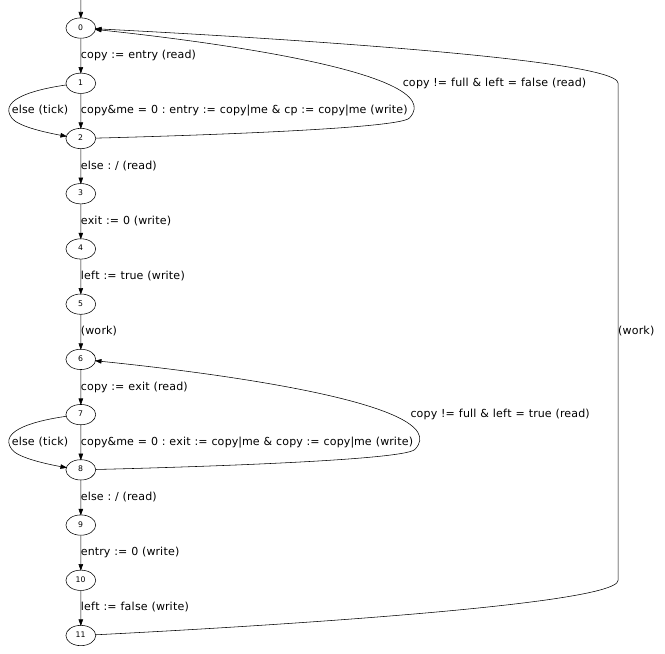
\includegraphics[width=5.2in]{ctmc}
	\caption{Continuous-time Markov chain model of the protocol}
	\label{fig:ctmc}
\end{figure}
\clearpage
\subsection{Modeling a cache line copy}
The following description shows a very simple view on the CPU cache and omits many details of current cache protocols. This is necessary to keep the model at a manageable size.

Each CPU core has its own copy of a cache line in its local cache. A copy of a cache line has three distinct states. It can be \emph{modified}, which means the core has the only up-to-date copy of the cache line and all other copies are marked \emph{invalid}. It might be \emph{shared}, which means the core has an up-to-date copy, but one or more other cores have a correct copy, too. Or the cache line copy is \emph{invalid}, meaning the local copy is not up-to-date. Figure~\ref{fig:cache} shows how a cache line copy changes its state depending on events occurring. The dotted transitions are triggered by events (read/write) occurring on other cores, whereas the solid transitions are due to events on the core itself.
\begin{figure}[htbp]
	\centering
	\includegraphics[width=2.7in]{cache}
	\caption{Model of the cache behaviour}
	\label{fig:cache}
\end{figure}

For example if a core reads a variable, it first needs to make sure that all other cores take notice and change its cache line copy state to shared in case it was modified before. After this the core fetches the cache line, marks it shared and continues reading the variable.

The timings of read and write are as follows. A read on a modified or shared variable does not imply any extra work but using the cached data. Therefore we consider this operation instantaneous. If a read is done on an invalid copy, it has to first fetch an up-to-date copy of the cache line and make sure all other cores are notified, until it can proceed. Therefor this operation takes usually around 50 CPU cycles. A write on a modified variable is instantaneous, since all other cores do not have an up-to-date copy and therefor do not have to be contacted. If the cache line in question is in a shared or invalid state, we first have to wait until all other cores follow the request to invalidate their copies of the  cache line. After this we can safely write to our local copy. This operation usually takes around 100 cycles.

The number of cycles those operations need is strongly dependent on the CPU itself. For the model we assume a cache read to use 50 cycles and a cache write to use 100 cycles.
\subsection{Properties}
We are interested to predict how long the barrier operation takes to complete. Therefore the following three property have been chosen.
\begin{enumerate}
	\item How long does it take for one thread to pass the barrier
	\item How long does it take for all threads to pass the barrier
	\item If one thread has left the barrier, how long does it take until all of them complete the barrier
\end{enumerate}

To formalise the above properties we use a continuous stochastic logic\cite{assb96}\cite{bkh99} representation. For the third query we use the \emph{conditional long-run probability}, which is explained in detail in \cite{fmix}.
\begin{enumerate}
	\item $P=? [\diamond_{\le t} \bigvee_{1 \le i \le n} loc_i \ge 5]$
	\item $P=? [\diamond_{\le t} \bigwedge_{1 \le i \le n} loc_i \ge 5]$
	\item $CrlP=? [\diamond_{\le t} \bigwedge_{1 \le i \le n} loc_i \ge 5, \bigvee_{1 \le i \le n} (l_i \ge 5 \wedge \bigwedge_{1 \le j \le n, i \neq j} l_j < 5)]$
\end{enumerate}
\subsection{Evaluation}
\begin{figure}[htbp]
	\centering
	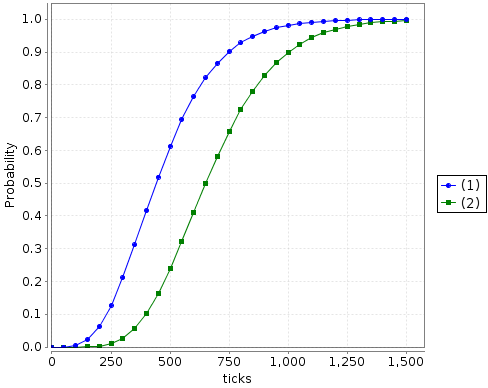
\includegraphics[width=3in]{one-and-all}
	\caption{Model checking results of query 1 and 2}
	\label{fig:one-and-all}
\end{figure}
\begin{figure}[htbp]
	\centering
	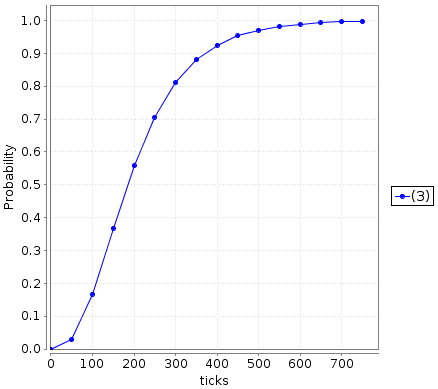
\includegraphics[width=3in]{one2all}
	\caption{Results of query 3}
	\label{fig:one2all}
\end{figure}

Note that for these queries the duration of the work period has few influence and is set to 1 cycle.

%%%%%%%%%%%%%%%%%%%%%%%%%%%%%%%%%%%%%%%%%%%%%%%%%%%%%%%%%%%%%%%%%%%%%%%%%%%%%%%
\section{Implementation and measurement}
\subsection{Considerations}
\subsection{Implementation}
\subsection{Evaluation}

%%%%%%%%%%%%%%%%%%%%%%%%%%%%%%%%%%%%%%%%%%%%%%%%%%%%%%%%%%%%%%%%%%%%%%%%%%%%%%%
\section{Conclusion}
\subsection{Lessons learned}
\subsection{Future Work}
\begin{itemize}
	\item reduce model
		\begin{itemize}
		\item symmetry
		\item query specific
			\begin{itemize}
				\item shorten second loop to just trigger cache state change from time to time
			\end{itemize}
		\item others?
		\end{itemize}
	\item implement
		\begin{itemize}
			\item GNU openmp
		\end{itemize}
	\item optimize
		\begin{itemize}
			\item use mwait or perhaps usleep()
			\item keep track who you personally have seen already in the barrier and him, too
		\end{itemize}
	\item evaluate for making it work for more than 32 processes
\end{itemize}


%%%%%%%%%%%%%%%%%%%%%%%%%%%%%%%%%%%%%%%%%%%%%%%%%%%%%%%%%%%%%%%%%%%%%%%%%%%%%%%
\nocite{*} % give out non cited references
\bibliographystyle{abbrv}
\bibliography{references}{}

\end{document}
